%template1.tex
%The following LaTeX source file represents the simplest kind of slide presentation; no overlays, no included graphics. Substitute your favorite style for ``pascal''. To create the PDF file template1.pdf, (1) be sure to use the prosper class, then (2) execute the command latex template1.tex, and (3) the command dvipdf template1.dvi.

%%%%%%%%%%%%%%%%%%%%%%%%%%%%%%% template1.tex %%%%%%%%%%%%%%%%%%%%%%%%%%%%%%%%%%%
\documentclass[a4paper,blends,pdf,colorBG,slideColor]{prosper}
% definitions for slides for CSC544
% Lutz Hamel, (c) 2007

\hypersetup{pdfpagemode=FullScreen}

\usepackage{amssymb}
\usepackage{latexsym}
\usepackage{amsmath}
%\usepackage[usenames]{color}
\usepackage{xypic}


\newcommand{\term}[1]{\ensuremath{\mbox{\bf #1}}}
\newcommand{\nonterm}[1]{\ensuremath{\mbox{#1}}}
\newcommand{\ifstmt}[3]{\ensuremath{{\bf if}\; {#1}\;{\bf then}\;{#2}\;{\bf else}\;{#3}\;\term{end}}}
\newcommand{\whilestmt}[2]{\ensuremath{{\bf while}\; {#1}\;{\bf do}\;{#2}\; \term{end}}}
\newcommand{\funcstmt}[3]{\ensuremath{{\bf fun}\; {#1}\; {\bf is}\; {#2} \; {\bf return}\; {#3}}}
\newcommand{\syntaxset}[1]{\ensuremath{\mbox{\bf #1}}}
\newcommand{\orbar}{\;|\;}
\newcommand{\bs}[1]{\begin{slide}{#1}\ptsize{8}}
\newcommand{\es}{\end{slide}}
\newcommand{\co}{\,\colon\;}
\newcommand{\pair}[2]{\ensuremath{\langle {#1}, {#2} \rangle}}
\newcommand{\encode}[1]{\ensuremath{\langle {#1} \rangle}}
\newcommand{\mytab}{\makebox[.15in]{}}
%\newcommand{\abs}[1]{{\mid{#1}\mid}}
\newcommand{\abs}[1]{{|{#1}|}}
\newcommand{\ol}[1]{\overline{#1}}

\newcommand{\qaccept}{\ensuremath{q_{\mbox{\tiny accept}}}}
\newcommand{\qreject}{\ensuremath{q_{\mbox{\tiny reject}}}}
\newcommand{\accept}{{\em accept}}
\newcommand{\reject}{{\em reject}}

\newcommand{\machine}[1]{
	\begin{quote}
	{#1}
	\end{quote}
	}

\newcommand{\fdef}[1]{
	\begin{center}
	\fbox{
	\begin{minipage}{3.5in}
	{\bf Definition:}
	{#1}
	\end{minipage}
	}
	\end{center}
	}

\newcommand{\ftheorem}[1]{
	\begin{center}
	\fbox{
	\begin{minipage}{3.5in}
	{\bf Theorem:}
	{#1}
	\end{minipage}
	}
	\end{center}
	}

\newcommand{\flemma}[1]{
	\begin{center}
	\fbox{
	\begin{minipage}{3.5in}
	{\bf Lemma:}
	{#1}
	\end{minipage}
	}
	\end{center}
	}


\newcommand{\fframe}[1]{
	\begin{center}
	\fbox{
	\begin{minipage}{3.5in}
	{#1}
	\end{minipage}
	}
	\end{center}
	}

\newcommand{\nframe}[1]{
	\begin{center}
	\begin{minipage}{3.5in}
	{#1}
	\end{minipage}
	\end{center}
	}

\begin{document}
\bs{Context-Free Languages}

As pointed out before, the prototypical context-free language is
\[
L = \{a^nb^n \mid a,b \in \Sigma \mbox{ and } n \ge 0\}
\]
In order to accept strings in this language a machine has to remember how
many $a$'s it has seen so that it can match the number $b$'s with the number
of $a$'s.

One way to accomplish this is with a stack, given some input string $s \in L$:
\begin{itemize}
\item ensure that only $b$'s follow the last $a$ in $s$,
\item push all the $a$'s of $s$ onto the stack,
\item then pop one $a$ off the stack for each $b$,
\item once we have read all the input symbols of $s$ and the stack is empty and
we are in an accepting state, then accept $s$; otherwise reject.
\end{itemize}
\es


\bs{Pushdown Automaton}
\begin{center}
\includegraphics[height=50mm]{images/pda-schema.eps}
\end{center}
\es

\bs{Formal Def. of PDA}

{\bf Definition:} a {\bf\em  pushdown automaton} is a 6-tuple 
$(Q, \Sigma, \Gamma, \delta, q_0, F)$, where
\begin{enumerate}
\item $Q$ is the set of states,
\item $\Sigma$ is input alphabet,
\item $\Gamma$ is the stack alphabet,
\item $\delta\co Q \times \Sigma_{\epsilon}\times\Gamma_\epsilon \rightarrow P(Q\times\Gamma_\epsilon)$ is the transition function,
\item $q_0 \in Q$ is the start state, and
\item $F \subseteq Q$ is the set of accept states.
\end{enumerate}
\vspace{.2in}
Is this a deterministic or nondeterministic machine?

\es

\bs{Formal Computation of PDA}
\begin{center}
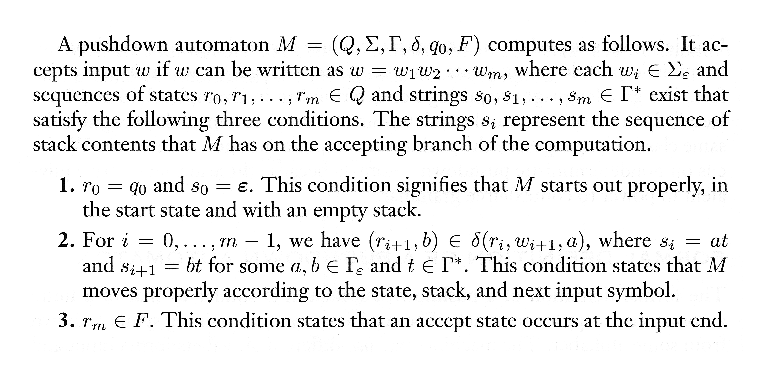
\includegraphics[height=50mm]{images/pda-computation.eps}
\end{center}
\es

\bs{$\{0^n1^n\mid n \ge 0\}$}

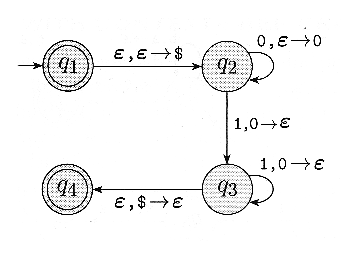
\includegraphics[height=20mm]{images/pda-01.eps}
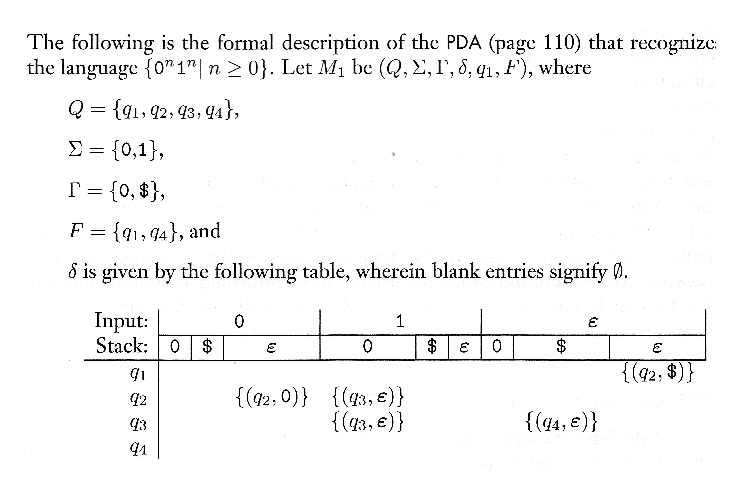
\includegraphics[height=50mm]{images/pda-01-desc.eps}


\es

\bs{Context-Free Languages}

\fframe{{\bf Definition:} A language is {\bf context-free} if some pushdown automaton recognizes it.}
\es

\bs{Context-Free Grammars}
\begin{center}
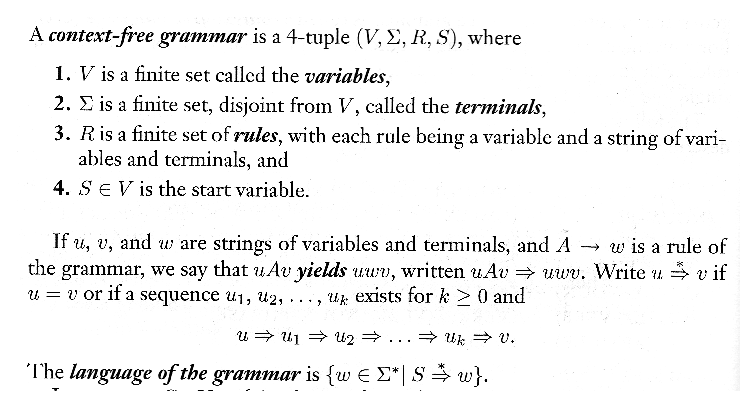
\includegraphics[height=55mm]{images/cfg-def.eps}
\end{center}
\es

\bs{Context-Free Grammars}
{\bf Example:} Given the context-free grammar $G = (V,\Sigma,R,S)$, with
$V = \{ A \}, \Sigma = \{a, b\}, S = A$, and $R$ the set of rules,
\begin{eqnarray*}
A &\rightarrow & a A b\\
A &\rightarrow & \epsilon
\end{eqnarray*}
then $L(G) = \{a^nb^n \mid n \ge 0\}$.
\es


\bs{CFL Theorem}

\vspace{.2in}
\begin{center}
\fbox{{\bf Theorem:} A language is context-free iff some context-free grammar (CFG) generates it.}
\end{center}
\vspace{.5in}
{\bf Proof Sketch:}\footnote{A related formal proof appears in the book; pp106ff 1st ed., pp115ff 2nd ed.)} Let $L$ be some language.
\begin{description}
\item[If $L$ is context-free, then some CFG generates it.]  If $L$ is context-free
then some PDA recognizes it.  We can show that for every PDA we can build a CFG that generates the language the PDA recognizes.
\item[If some CFG generates  $L$, then $L$ is context-free.] For every CFG that
generates $L$ we
can show that we can construct a PDA that recognizes $L$.
\end{description}
\vspace{.2in}
\es

\bs{Language Hierarchy}

\begin{center}
\framebox{{\bf Corollary:} Every regular language is also a context-free language.}
\end{center}

{\bf Proof Sketch:} A PDA can simulate an FA by ignoring its stack.

This gives us the following hierarchy of languages
\begin{center}
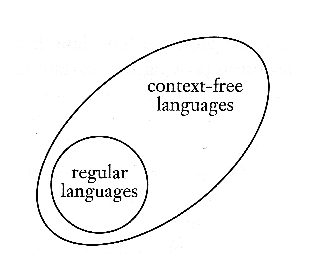
\includegraphics[height=40mm]{images/hierarchy-1.eps}
\end{center}
\es


\bs{Chomsky Normal Form}

The Chomsky normal form of a context free grammar is convenient to work with, especially later when we want to 
prove properties of context-free languages.

{\bf Definition:} A context-free grammar $(V,\Sigma,R,s)$ is in Chomsky normal form if every rule in $R$ is of the form
\begin{eqnarray*}
A &\rightarrow& BC\\
A&\rightarrow& a
\end{eqnarray*}
with$a,B,C \in V$ and $a\in\Sigma$.
\es

\bs{Chomsky Normal Form}

\fframe{{\bf Theorem:} Any context-free language is generated by a context-free grammar in Chomsky normal form}

{\bf Proof Sketch:} Any context-free grammar can be converted to a grammar in Chomsky normal form.
\es

\bs{Chomsky Normal Form}

{\bf Example:} Convert the following CFG to Chomsky Normal Form (CNF):
\begin{eqnarray*}
S&\rightarrow& aX | Yb\\
X&\rightarrow& S | \epsilon\\
Y&\rightarrow& bY | b
\end{eqnarray*}
{\bf Step 1} - Kill all $\epsilon$ productions:
By inspection, the only nullable nonterminal is $X$.
Delete all $\epsilon$ productions and add new productions, with all possible
combinations of the nullable $X$ removed.
The new CFG, without $\epsilon$ productions, is:
\begin{eqnarray*}
S&\rightarrow& aX | a | Yb\\
X&\rightarrow&S\\
Y&\rightarrow&bY | b
\end{eqnarray*}
\es

\bs{Chomsky Normal Form}

{\bf Step 2} - Kill all unit productions:
The only unit production is $X\rightarrow S$, where the $S$ can be replaced with all
$S$�s non-unit productions (i.e. $aX$, $a$, and $Yb$).
The new CFG, without unit productions, is:
\begin{eqnarray*}
S&\rightarrow&aX | a | Yb\\
X&\rightarrow&aX | a | Yb\\
Y&\rightarrow&bY | b
\end{eqnarray*}
{\bf Step 3} - Replace all mixed strings with solid nonterminals.
Create extra productions that produce one terminal, when doing the
replacement.
The new CFG, with a RHS consisting of only solid nonterminals or one
terminal is:
\begin{eqnarray*}
S&\rightarrow&AX | YB | a\\
X&\rightarrow&AX | YB | a\\
Y&\rightarrow&BY | b\\
A&\rightarrow&a\\
B&\rightarrow& b
\end{eqnarray*}
\es

\bs{Beyond CFL's}

Are there languages beyond context-free languages?  Yes, consider
\[
L = \{ a^nb^nc^n \mid a,b,c \in \Sigma \mbox{ and } n \ge 0 \}.
\]
Our stack approach does not work anymore because we need to keep track
of three entities.

\es

\bs{CFL Pumping Lemma}
\ftheorem{{[Pumping Lemma for Context-free Languages]} If $A$ is a context-free language
then there is a number $p$ (the pumping length) where, if $s$ is any string $A$ of length at least $p$, then $s$
may be divided into five pieces $s = uvxyz$ satisfying the conditions
\begin{enumerate}
\item for each $i \ge 0$, $uv^ixy^iz \in A$,
\item $| vy | > 0$,
\item $| vxy | \le p$.
\end{enumerate}
}
\es


\bs{CFL Pumping Lemma}
As before we can use the pumping lemma to show that certain languages are {\em not} context-free.

\ftheorem{The language $A =\{ a^nb^nc^n \mid n \ge 0\}$ is not context free.}

{\bf Proof:} Proof by contradiction using the pumping lemma.  If the language is context free then there should be
some string $s \in A$ with $|s| \ge p$ where $p$ is the pumping length.  Let $s = a^pb^pc^p$ be that string.
The pumping lemma state that we can split up the string into $s = uvxyz$ such that $uv^ixy^iz \in A$ for all $i \ge 0$.
Given conditions 2 and 3 of the pumping lemma this is clearly not possible.
$\Box$
\es

\bs{CFL Pumping Lemma}
{\bf Observations:} Where does the pumping length come from? We cannot use a pumping length derived from 
the PDA because the PDA now contains an infinite structure making the argument of a forced looping given 
a string with the length of at least the number states difficult.

However, we can look at looping during derivations in grammars. 
\es


\bs{CFL Pumping Lemma}

Consider the following grammar in Chomsky normal form of the language $L =\{ a^n \mid n >0\}$,
{\scriptsize
\begin{eqnarray*}
A &\rightarrow& AA\\
A &\rightarrow& a
\end{eqnarray*}
}
The longest string we can generate without repeating a rule from the start symbol to a leaf node is `$aa$',

{\scriptsize
\[
\xymatrix{
&A\ar[ld]\ar[rd] &  \\
A\ar[d]&&A\ar[d]\\
a & & a
}
\]
}

That means, the derivation of any string with a length $> 2$ will force a {\em recursive} application of the first rule --
that is, the derivation loops!  But this would also mean that the associated PDA would loop!
\es

\bs{CFL Pumping Lemma}
Also notice that for a grammar in Chomsky normal form the length of a generated string $s$ is related to the 
levels $t$ in the derivation tree as
\[
|s| \le 2^t
\]
We can relate this back to the number of non-terminals: Let $V$ be the set of non-terminals in the grammar, then
$|V|$ is the maximum number of levels in a parse tree without repeating a rule in any branch.  Or in other words,
if 
\[
|s| > 2^{|V|}
\]
then one of its branches will have a repeated rule.

Check that in the grammar above.
\es

\bs{CFL Pumping Lemma}
{\bf Example:} Consider the grammar in Chomsky normal form for the language 
\[
L = \{a^nb^n \mid n > 0\},
\]
\begin{eqnarray*}
A & \rightarrow & AP \\
P & \rightarrow & QB \\
Q & \rightarrow & AP \\
A & \rightarrow & a\\
B & \rightarrow & b \\
P & \rightarrow & b
\end{eqnarray*}
Observe that $V = \{A,B,P,Q\}$, that is, strings with length $\ge 2^4$ will be generated using repeated rules.
\es

\bs{CFL Pumping Lemma}

{\bf Proposition:} CFGs with recursive rules have a pumping length.

{\bf Proof:} Follows directly from the fact that any CFG can be written in Chomsky Normal Form and that derivations
in Chomsky Normal Form grammars are binary trees.

\es

\bs{CFL Pumping Lemma}
{\bf Example:} Consider the CFG for the language 
\[
L = \{a^nb^n \mid n > 0\},
\]
\begin{eqnarray*}
S & \rightarrow & ASB \\
S & \rightarrow & \epsilon\\
A & \rightarrow & a\\
B & \rightarrow & b
\end{eqnarray*}
\es

\end{document}
%%%%%%%%%%%%%%%%%%%%%%%%%%% end of template1.tex %%%%%%%%%%%%%%%%%%%%%%%%%%%%%%%%

